% -*- coding: utf-8 -*-
\documentclass[UTF8,a4paper,10pt]{ctexart}
\usepackage[left=3.17cm, right=3.17cm, top=2.74cm, bottom=2.74cm]{geometry}
\usepackage{amsmath}
\usepackage{amssymb}
\usepackage{graphicx}
\usepackage{float}
\usepackage{booktabs}
\usepackage{multirow}
\usepackage{caption}
\usepackage{subcaption}
\usepackage{tabularx}
\usepackage{array}
\usepackage{makecell}
\usepackage{enumerate}
\usepackage{enumitem}
\usepackage{xcolor}
\usepackage{listings}
\usepackage[most]{tcolorbox}
\usepackage[colorlinks,linkcolor=black,anchorcolor=blue,hypertexnames=false]{hyperref}
\usepackage{fancyhdr}
\usepackage{tikz}
\usetikzlibrary{fit, positioning, arrows.meta, calc, backgrounds}
\usepackage{eso-pic}

%-------------------------字体设置--------------
\newcommand{\yihao}{\fontsize{26pt}{36pt}\selectfont}
\newcommand{\erhao}{\fontsize{22pt}{28pt}\selectfont}
\newcommand{\xiaoer}{\fontsize{18pt}{18pt}\selectfont}
\newcommand{\sanhao}{\fontsize{16pt}{24pt}\selectfont}
\newcommand{\xiaosan}{\fontsize{15pt}{22pt}\selectfont}
\newcommand{\sihao}{\fontsize{14pt}{21pt}\selectfont}
\newcommand{\xiaosi}{\fontsize{12pt}{20pt}\selectfont}
\newcommand{\wuhao}{\fontsize{10.5pt}{15.75pt}\selectfont}
% 架构图节点内的灰色小号子标签（声明式，作用至所在单元行末）
\newcommand{\sub}{\normalfont\scriptsize\color{gray!60}}

%-------------------------章节名----------------
\ctexset{
  section = {
    name = {,、},
    number = \chinese{section}
  },
  subsection = {
    name = {（,）},
    number = \chinese{subsection}
  },
  subsubsection = {
    name = {,},
    number = \arabic{subsubsection}.
  }
}

%-------------------------页眉页脚--------------
\pagestyle{fancy}
\lhead{\kaishu \leftmark}
\rhead{\kaishu 推荐系统评分预测实验报告}
\lfoot{}
\cfoot{\thepage}
\rfoot{}
\renewcommand{\headrulewidth}{0.1pt}
\renewcommand{\footrulewidth}{0pt}
\newcommand{\HRule}{\rule{\linewidth}{0.5mm}}
\newcommand{\HRulegrossa}{\rule{\linewidth}{1.2mm}}

%------------------------代码-------------------
\lstset{
breaklines=true,
breakatwhitespace=false,
columns=flexible,
basicstyle=\small\ttfamily,
escapeinside={(*@}{@*)},
keywordstyle=\color[RGB]{0,0,180}\bfseries,
commentstyle=\color[RGB]{106,153,85},
stringstyle=\color[RGB]{163,21,21},
extendedchars=false,
linewidth=\textwidth,
numbers=left,
numberstyle=\tiny \color{blue!50},
frame=trbl,
rulesepcolor=\color{red!20!green!20!blue!20},
captionpos=b
}
\DeclareCaptionFormat{lstnocounter}{\small\textbf{代码\thelstlisting：#3}}
\captionsetup[lstlisting]{format=lstnocounter, singlelinecheck=true, skip=2pt, justification=centering}
\setlength{\emergencystretch}{3em}
\hbadness=2000
\newcolumntype{Y}{>{\raggedright\arraybackslash}X}

%------------------------水印-------------------
\newcommand{\watermark}[3]{\AddToShipoutPictureBG{
\parbox[b][\paperheight]{\paperwidth}{
\vfill
\centering
\tikz[remember picture, overlay]
  \node [rotate = #1, scale = #2] at (current page.center)
    {\textcolor{gray!80!cyan!30!magenta!30}{#3}};
\vfill}}}

\begin{document}
\begin{titlepage}
  \begin{center}
    
\includegraphics[width=0.68\textwidth]{NKU.png}\\[0.35cm]
    {\Huge \kaishu 南\ \ \ \ \ \ 开\ \ \ \ \ \ 大\ \ \ \ \ \ 学}\\[0.35cm]
    {\Large \textbf{大数据计算课程第二次作业}}\\[0.35cm]
    \HRule \\[0.35cm]
    { \LARGE \bfseries 推荐系统评分预测实验报告}\\[0.3cm]
    \HRule \\[0.65cm]
    {\small \kaishu
    \renewcommand{\arraystretch}{1.22}
    \begin{tabularx}{0.96\textwidth}{>{\centering\arraybackslash}X|>{\centering\arraybackslash}X|>{\centering\arraybackslash}X}
      \textbf{成员一} & \textbf{成员二} & \textbf{成员三} \\
      \hline
      密码与网络空间安全学院 & 计算机学院 & 计算机学院 \\
      2023级 & 2023级 & 2023级 \\
      信息安全班 & 计算机科学卓越班 & 计算机科学卓越班 \\
      2311208 & 2310428 & 2311671 \\
      魏来 & 韩琦卓 & 侯嘉栋 \\
    \end{tabularx}}\\[0.35cm]
    \vfill
    {\Large \today}
  \end{center}
\end{titlepage}

\tableofcontents
\newpage
\watermark{60}{10}{NKU}
\setcounter{page}{1}

% ============================================================
\section{实验摘要}
\xiaosi

\begin{tcolorbox}[colback=blue!3!white,colframe=blue!55!black,title=核心结论]
  本实验选择任务一，在 \texttt{train.txt} 上实现带偏置矩阵分解（Biased SVD / FunkSVD）进行显式评分预测。模型预测公式为 $\hat{r}_{ui} = \mu + b_u + b_i + \mathbf{p}_u \cdot \mathbf{q}_i$，以 SGD 优化带 L2 正则的平方损失，并结合收缩偏置热启动、10\% 验证集早停与两阶段再训练策略。最终模型在验证集上 RMSE 为 \textbf{17.024}，相较全局均值基线（RMSE = 20.81）改善约 \textbf{18.2\%}；预测结果已按 ResultForm 格式写入 \texttt{result/prediction.txt}。
\end{tcolorbox}

\begin{table}[H]
  \centering
  \caption{实验关键指标一览}
  \begin{tabular}{c c c c c c}
    \toprule
    \textbf{训练样本} & \textbf{验证样本} & \textbf{测试对数} & \textbf{最优轮次} & \textbf{验证集 RMSE} & \textbf{运行时间} \\
    \midrule
    81,769 & 9,085 & 9,982 & 54 & 17.024 & 71.3 s \\
    \bottomrule
  \end{tabular}
\end{table}

% ============================================================
\section{实验目的}
\xiaosi

推荐系统是大数据时代最重要的应用之一，其核心任务是根据用户的历史行为预测用户对未见物品的偏好程度。显式评分预测是最基础的推荐子任务，要求直接预测用户对物品的数值评分。本次实验围绕课程给定的 \texttt{train.txt} / \texttt{test.txt} 数据集，实现基于带偏置矩阵分解的评分预测系统，主要目标如下：

\begin{enumerate}
  \item 理解矩阵分解推荐模型的数学原理，掌握用户偏置、物品偏置和隐向量协同描述评分模式的方法。
  \item 从零实现带正则的 SGD 优化流程，理解学习率、L2 正则系数、早停耐心等超参数对训练的影响。
  \item 使用数值收缩偏置热启动，加速偏置项收敛，降低训练初期对稀疏数据的过拟合风险。
  \item 设计两阶段再训练策略：第一阶段在 90\% 训练集上通过早停确定最优轮次；第二阶段在全部训练数据上按最优轮次进行再训练，充分利用所有可用数据。
  \item 分析评分分布特征、物品受欢迎度对预测精度的影响，理解冷启动问题的处理方式。
\end{enumerate}

% ============================================================
\section{实验内容}
\xiaosi

本实验完成的核心工作包括：

\begin{enumerate}
  \item 解析 \texttt{train.txt} 数据文件（用户--物品--评分三元组）与 \texttt{test.txt} 文件（用户--物品对），理解数据分布特征。
  \item 统计数据集基础特征：评分分布（离散值 10, 20, \ldots, 100）、用户活跃度分布（幂律长尾）、物品受欢迎度分布。
  \item 将评分从 $[10, 100]$ 归一化到 $[1, 10]$ 后在归一化空间中训练，预测时反归一化并裁剪到合法评分范围。
  \item 使用收缩偏置（Koren 2009 §2.1）对用户偏置和物品偏置进行热启动，减少数据稀疏引起的训练不稳定性。
  \item 随机划分 10\% 的训练评分为验证集，进行早停（patience = 5），记录最优轮次 $N^* = 54$。
  \item 再训练阶段使用全部训练评分（不含测试标签）对模型进行 $N^*$ 轮 SGD 优化，使最终预测得益于更多的监督信号。
  \item 对不同超参数组合（隐向量维度、L2 正则系数）进行网格搜索，记录各配置验证集 RMSE。
  \item 按 \texttt{ResultForm.txt} 规定格式写出 \texttt{result/prediction.txt}，并记录 \texttt{result/metrics.json}。
\end{enumerate}

% ============================================================
\section{数据集描述}
\xiaosi

\subsection{数据格式}

本实验使用课程给定的任务一数据集。训练文件 \texttt{data/train.txt} 采用如下格式：

\begin{lstlisting}[language=bash, caption={train.txt 数据格式}]
<user_id>|<count>
<item_id>   <score>
...
\end{lstlisting}

其中每个用户块以 \texttt{user\_id|count} 开头，后跟该用户的 \texttt{count} 条评分记录。测试文件 \texttt{data/test.txt} 格式相同，但评分列省略，需预测该列。评分值是离散值，合法取值为 $\{10, 20, 30, 40, 50, 60, 70, 80, 90, 100\}$，代表 10\% 粒度的百分制评分。

\subsection{基础统计}

\begin{table}[H]
  \centering
  \caption{数据集基础统计信息}
  \begin{tabular}{cc}
    \toprule
    \textbf{统计项} & \textbf{值} \\
    \midrule
    训练集总评分数 & 90,854 \\
    用户数 & 598 \\
    物品数 & 9,077 \\
    评分均值 & 69.9 \\
    评分标准差 & 20.8 \\
    评分众数 & 80 \\
    最大用户评分数 & 2,678 \\
    最大物品被评次数 & 251 \\
    仅出现 1 次的物品数（冷启动） & 1,647 \\
    测试对数 & 9,982 \\
    \bottomrule
  \end{tabular}
\end{table}

\begin{figure}[H]
  \centering
  
\includegraphics[width=\textwidth]{images/dataset_overview.png}
  \caption{数据集总览：评分分布、用户活跃度分布（对数尺度）与物品受欢迎度分布（对数尺度）}
  \label{fig:dataset-overview}
\end{figure}

\begin{tcolorbox}[colback=cyan!5!white,colframe=cyan!75!black,title=数据集特征分析]
  \hspace{2em}图~\ref{fig:dataset-overview} 面板 A 展示了离散评分的频率分布，分数 80 出现频率最高（约 19,000 次），整体分布右偏，高分频次较多。面板 B 和 C 分别以对数尺度展示用户活跃度和物品受欢迎度，两者均呈现出典型的幂律长尾分布：少数活跃用户和少数热门物品贡献了大量评分，而多数用户和物品的评分次数极少。这种长尾特性是推荐系统中冷启动问题的根源，也是评估模型鲁棒性的重要维度。
\end{tcolorbox}

% ============================================================
\section{实验原理}
\xiaosi

\subsection{带偏置矩阵分解模型}

矩阵分解推荐模型的核心思想是将用户--物品评分矩阵 $R\in\mathbb{R}^{|U|\times|I|}$ 分解为若干低秩因子的乘积，以捕捉用户偏好与物品特征之间的隐含相关性。设全局评分均值为 $\mu$，用户 $u$ 的偏置为 $b_u$（反映该用户打分习惯的高低），物品 $i$ 的偏置为 $b_i$（反映该物品总体受欢迎程度），用户 $u$ 的隐向量为 $\mathbf{p}_u\in\mathbb{R}^F$，物品 $i$ 的隐向量为 $\mathbf{q}_i\in\mathbb{R}^F$，则带偏置矩阵分解（Biased SVD / FunkSVD，Koren 2009）的预测公式为：

\begin{equation}
  \hat{r}_{ui} = \mu + b_u + b_i + \mathbf{p}_u \cdot \mathbf{q}_i
  \label{eq:biasedsvd}
\end{equation}

其中 $F$ 为隐向量维度（本实验取 $F=100$）。四个项的物理含义可解释为：$\mu$ 捕捉全局打分水平，$b_u$ 捕捉用户级别的打分偏高或偏低倾向，$b_i$ 捕捉物品自身的总体口碑效应，$\mathbf{p}_u\cdot\mathbf{q}_i$ 捕捉用户--物品间的个性化交互。

\begin{figure}[H]
  \centering
  \resizebox{\textwidth}{!}{%
  \begin{tikzpicture}[>=stealth, thick, font=\small,
    stage/.style={draw=gray!45, dashed, rounded corners, inner sep=10pt},
    box/.style={draw, rounded corners=3pt, align=center,
                minimum width=2.2cm, minimum height=0.95cm},
    inp/.style={box, fill=gray!8},
    ublk/.style={box, fill=blue!7},
    iblk/.style={box, fill=orange!10},
    inter/.style={box, fill=violet!10},
    agg/.style={box, fill=green!8},
    uedge/.style={->, blue!60!black},
    iedge/.style={->, orange!75!black},
    medge/.style={->, green!45!black}]

    % --- Input ---
    \node[inp] (user) at (0, -1.0) {用户 $u$};
    \node[inp] (item) at (0, -4.2) {物品 $i$};

    % --- Embedding lookup ---
    \node[ublk] (bu) at (3.4,  0.4) {$b_u$\\[1pt]\sub 用户偏置};
    \node[ublk] (pu) at (3.4, -1.4) {$\mathbf{p}_u$\\[1pt]\sub 用户隐向量};
    \node[iblk] (bi) at (3.4, -3.4) {$b_i$\\[1pt]\sub 物品偏置};
    \node[iblk] (qi) at (3.4, -5.2) {$\mathbf{q}_i$\\[1pt]\sub 物品隐向量};

    % --- Interaction ---
    \node[inter] (dot) at (7.1, -3.3)
      {$\mathbf{p}_u\!\cdot\!\mathbf{q}_i$\\[1pt]\sub 内积（标量）};

    % --- Aggregate ---
    \node[agg] (mu) at (10.3, 0.6) {$\mu$\\[1pt]\sub 全局均值};
    \node[agg, circle, minimum width=1.1cm] (sum) at (10.3, -2.0) {$\Sigma$};

    % --- Output ---
    \node[agg] (clip) at (13.3, -2.0) {裁剪 $[10,100]$};
    \node[agg] (out)  at (13.3, -4.4) {$\hat{r}_{ui}$};

    % --- Stage frames ---
    \node[stage, fit=(user)(item), label={[font=\bfseries]above:输入}] {};
    \node[stage, fit=(bu)(pu)(bi)(qi), label={[font=\bfseries]above:嵌入查找}] {};
    \node[stage, fit=(dot), label={[font=\bfseries]above:特征交互}] {};
    \node[stage, fit=(mu)(sum), label={[font=\bfseries]above:加权汇总}] {};
    \node[stage, fit=(clip)(out), label={[font=\bfseries]above:输出}] {};

    % --- Edges ---
    \draw[uedge] (user) -- (bu);
    \draw[uedge] (user) -- (pu);
    \draw[iedge] (item) -- (bi);
    \draw[iedge] (item) -- (qi);
    \draw[uedge] (pu) -- (dot);
    \draw[iedge] (qi) -- (dot);
    \draw[uedge] (bu.east) -- (sum);
    \draw[iedge] (bi.east) -| ([xshift=-2pt]sum.south);
    \draw[->, violet!60!black] (dot) -- (sum);
    \draw[medge] (mu) -- (sum);
    \draw[medge] (sum) -- (clip);
    \draw[medge] (clip) -- (out);
  \end{tikzpicture}}
  \caption{Biased SVD 模型结构：从用户 $u$ 和物品 $i$ 到预测评分 $\hat{r}_{ui}$ 的完整计算路径}
  \label{fig:model-arch}
\end{figure}

\begin{tcolorbox}[colback=blue!3!white,colframe=blue!55!black,title=模型设计说明]
  \hspace{2em}图~\ref{fig:model-arch} 展示了 Biased SVD 的计算图。用户 $u$ 通过嵌入查找得到用户偏置 $b_u$ 和用户隐向量 $\mathbf{p}_u$；物品 $i$ 同样得到物品偏置 $b_i$ 和物品隐向量 $\mathbf{q}_i$。内积 $\mathbf{p}_u\cdot\mathbf{q}_i$ 经过加法节点 $\Sigma$ 将四项（$\mu, b_u, b_i, \mathbf{p}_u\cdot\mathbf{q}_i$）汇总，再经裁剪层限制到 $[10, 100]$ 范围得到最终预测 $\hat{r}_{ui}$。
\end{tcolorbox}

\subsection{目标函数与 SGD 优化}

模型在归一化评分空间（$\tilde{r} = r / 10$，对应范围 $[1, 10]$）中训练，全局均值 $\tilde{\mu}$ 也在归一化空间计算。训练目标为最小化带 L2 正则的均方损失：

\begin{equation}
  \mathcal{L} = \sum_{(u,i,r)\in\mathcal{D}} \bigl(\tilde{r}_{ui} - \tilde{\mu} - b_u - b_i - \mathbf{p}_u\cdot\mathbf{q}_i\bigr)^2
  + \lambda\bigl(\|b_u\|^2 + \|b_i\|^2 + \|\mathbf{p}_u\|^2 + \|\mathbf{q}_i\|^2\bigr)
  \label{eq:loss}
\end{equation}

其中 $\lambda$ 为正则化系数（本实验取 $\lambda = 0.2$）。对每条训练评分 $(u, i, \tilde{r})$，定义预测误差 $e_{ui} = \tilde{r} - (\tilde{\mu} + b_u + b_i + \mathbf{p}_u\cdot\mathbf{q}_i)$，SGD 更新规则为：

\begin{align}
  b_u &\leftarrow b_u + \eta\,(e_{ui} - \lambda\,b_u) \label{eq:update-bu}\\
  b_i &\leftarrow b_i + \eta\,(e_{ui} - \lambda\,b_i) \label{eq:update-bi}\\
  \mathbf{p}_u &\leftarrow \mathbf{p}_u + \eta\,(e_{ui}\,\mathbf{q}_i - \lambda\,\mathbf{p}_u) \label{eq:update-pu}\\
  \mathbf{q}_i &\leftarrow \mathbf{q}_i + \eta\,(e_{ui}\,\mathbf{p}_u - \lambda\,\mathbf{q}_i) \label{eq:update-qi}
\end{align}

其中 $\eta$ 为学习率（本实验取 $\eta = 0.005$）。注意更新 $\mathbf{q}_i$ 时使用更新前的 $\mathbf{p}_u$（先保存副本），以保证两个方向梯度的独立性。

\subsection{收缩偏置热启动}

直接随机初始化偏置项在数据稀疏情况下容易产生高方差估计。本实验采用 Koren（2009）第 2.1 节的收缩偏置估计对 $b_u$ 和 $b_i$ 进行热启动：

\begin{align}
  \hat{b}_i &= \frac{\displaystyle\sum_{u\in R(i)} (\tilde{r}_{ui} - \tilde{\mu})}{\lambda_i + |R(i)|} \label{eq:shrink-bi}\\[6pt]
  \hat{b}_u &= \frac{\displaystyle\sum_{i\in R(u)} (\tilde{r}_{ui} - \tilde{\mu} - \hat{b}_i)}{\lambda_u + |R(u)|} \label{eq:shrink-bu}
\end{align}

其中 $|R(i)|$ 为物品 $i$ 的评分数，$\lambda_i = 25$ 为物品收缩系数；$|R(u)|$ 为用户 $u$ 的评分数，$\lambda_u = 10$ 为用户收缩系数。对评分稀少的冷门物品，分母中的 $\lambda_i$ 将偏置强烈拉向 0；对评分较多的热门物品，$\lambda_i$ 的影响减弱，偏置估计趋向真实经验均值。

\subsection{冷启动处理}

测试集中可能出现训练集未见过的用户或物品（冷启动情形）。在预测时，若用户 $u$ 未知，则令 $b_u = 0$，$\mathbf{p}_u$ 对应项贡献为 0；若物品 $i$ 未知，则令 $b_i = 0$，$\mathbf{q}_i$ 贡献为 0。因此冷启动情形下预测退化为：

\begin{equation}
  \hat{r}_{ui} =
  \begin{cases}
    \mu + b_u & \text{物品未知（仅用用户偏置修正）} \\
    \mu + b_i & \text{用户未知（仅用物品偏置修正）} \\
    \mu        & \text{二者均未知}
  \end{cases}
\end{equation}

这种退化方案保证预测结果在任何情况下都是合理的，不会出现越界或 NaN。

% ============================================================
\section{算法设计}
\xiaosi

\subsection{两阶段再训练策略}

为同时利用早停机制（防止过拟合）和全量数据（减少估计方差），本实验采用两阶段训练策略：

\begin{figure}[H]
  \centering
  \resizebox{\textwidth}{!}{%
  \begin{tikzpicture}[>=stealth, thick, font=\small,
    box/.style={draw, rounded corners=3pt, align=center,
                minimum width=2.6cm, minimum height=1.5cm},
    data/.style={box, fill=cyan!7},
    tr/.style={box, fill=blue!7},
    va/.style={box, fill=orange!10},
    ph1/.style={box, fill=violet!9, minimum width=3.6cm, minimum height=2.7cm},
    ph2/.style={box, fill=green!8,  minimum width=3.6cm, minimum height=2.7cm},
    pred/.style={box, fill=green!10},
    lbl/.style={font=\scriptsize\itshape, text=gray!60,
                fill=white, inner sep=1.5pt},
    tag/.style={draw=violet!55, rounded corners=2pt, fill=violet!12,
                font=\scriptsize, inner sep=2.5pt}]

    \node[data] (raw) at (0,-1.8)
      {\textbf{train.txt}\\[3pt]\sub 90,854 条评分\\\sub 598 用户 · 9,077 物品};
    \node[tr] (train) at (4.2, -0.4)
      {\textbf{训练集（90\%）}\\[3pt]\sub 81,769 条};
    \node[va] (val) at (4.2, -3.2)
      {\textbf{验证集（10\%）}\\[3pt]\sub 9,085 条};

    \node[ph1] (p1) at (8.8, -1.8)
      {\textbf{阶段一 · 早停}\\[3pt]\sub 最多 60 轮 SGD\\\sub 监控验证集 RMSE
       \\\sub patience = 5\\\sub 最优轮次 $N^{*}=54$};
    \node[ph2] (p2) at (14.0, -1.8)
      {\textbf{阶段二 · 再训练}\\[3pt]\sub 全部 90,854 条\\\sub 固定 $N^{*}=54$ 轮
       \\\sub 不再使用验证集};
    \node[pred] (pred) at (14.0, -5.8)
      {\textbf{prediction.txt}\\[3pt]\sub 9,982 个测试对};

    % edges
    \draw[->, cyan!55!black] (raw.east) |- (train.west);
    \draw[->, cyan!55!black] (raw.east) |- (val.west);
    \draw[->, blue!60!black]   (train.east) -- (p1.west);
    \draw[->, orange!75!black, dashed]
      (val.east) -- node[lbl, pos=0.45]{仅监控} (p1.west);
    \draw[->, violet!60!black]
      (p1.east) -- node[tag, above=1pt]{$N^{*}=54$} (p2.west);
    \draw[->, green!45!black]
      (p2.south) -- node[lbl, right=1pt]{预测} (pred.north);
    % val data reused in phase 2 (clean lower lane)
    \draw[->, orange!70!black, dashed]
      (val.south) -- ++(0,-0.65) -| ([xshift=-0.6cm]p2.south);
    \node[lbl] at (9.0,-4.35) {全量数据于阶段二复用};

    % bottom note
    \node[draw=orange!60, rounded corners, fill=orange!6,
          text width=13.5cm, align=center, font=\small, inner sep=6pt]
      at (6.2, -7.3)
      {$\bigstar$\,验证集仅用于监控与早停，\textbf{从不参与梯度更新}（零数据泄漏）};
  \end{tikzpicture}}
  \caption{两阶段训练策略总览：第一阶段通过早停确定最优轮次，第二阶段用全量数据再训练}
  \label{fig:two-phase}
\end{figure}

\begin{enumerate}
  \item \textbf{第一阶段（早停）：} 从 90,854 条训练评分中随机抽取 10\% 作为验证集（9,085 条），剩余 81,769 条作为训练集。以最大 60 轮为上限执行 SGD，每轮结束后评估验证集 RMSE。若连续 5 轮（patience = 5）验证集 RMSE 不再下降，则停止训练并恢复最优 checkpoint 对应的参数。本次运行在第 54 轮取得最优验证集 RMSE = 17.024。

  \item \textbf{第二阶段（再训练）：} 将最优轮次 $N^* = 54$ 作为固定轮数，在全部 90,854 条训练评分上重新训练模型，不使用早停和验证集。再训练完成后，用得到的最终参数对测试集进行预测。
\end{enumerate}

\begin{tcolorbox}[colback=green!5!white,colframe=green!50!black,title=两阶段再训练的合理性]
  \hspace{2em}单纯的早停只利用了 90\% 的训练数据；直接在全量数据上训练固定轮数又缺乏自动确定合适轮次的机制。两阶段策略兼顾二者：第一阶段的验证集仅用于监控，不参与梯度更新（零数据泄漏），仅用于确定 $N^*$；第二阶段则将这 10\% 的评分重新纳入训练，弥补第一阶段因验证集拆分带来的样本损失。
\end{tcolorbox}

\subsection{训练收敛曲线}

\begin{figure}[H]
  \centering
  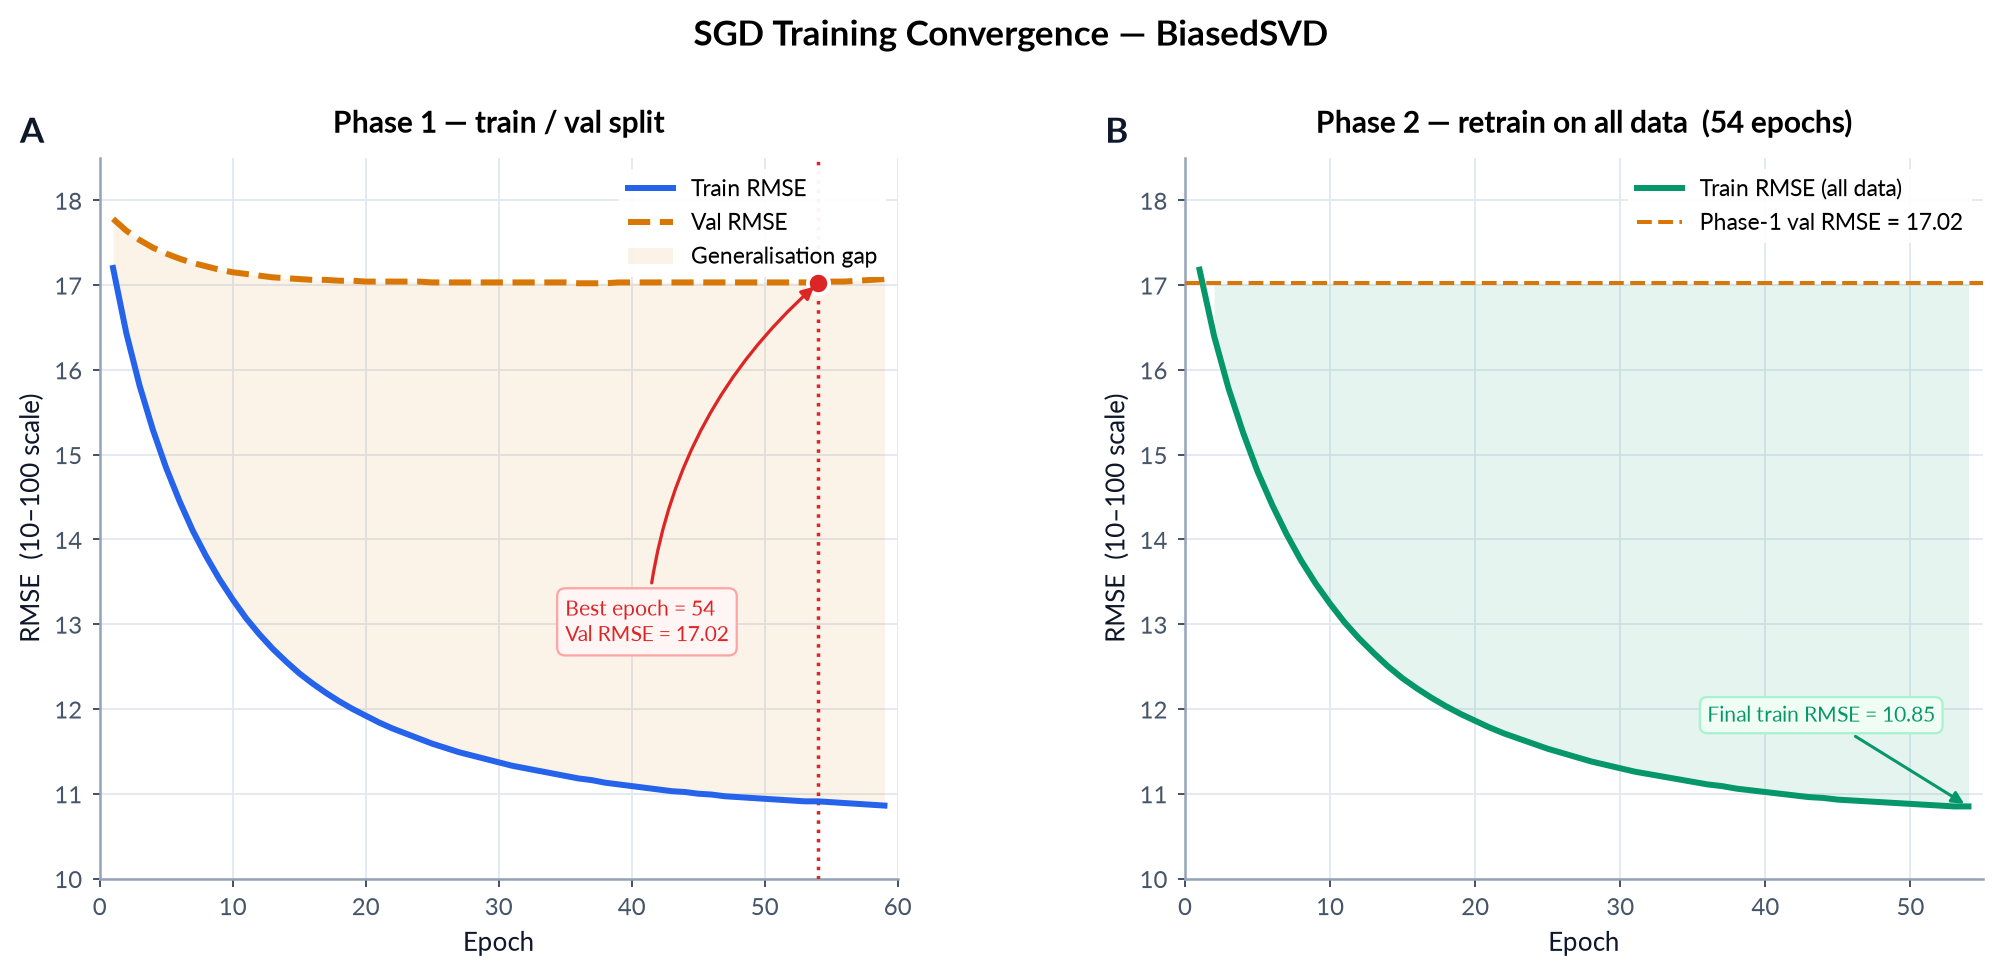
\includegraphics[width=\textwidth]{images/training_curve.png}
  \caption{SGD 训练收敛曲线：面板 A 为第一阶段（训练集/验证集 RMSE），面板 B 为第二阶段（全量数据）}
  \label{fig:training-curve}
\end{figure}

图~\ref{fig:training-curve} 面板 A 展示了第一阶段的训练曲线。训练 RMSE 随轮次单调下降，验证集 RMSE 在前 20 轮内快速收敛，随后进入缓慢优化阶段并在第 54 轮达到最低值 17.024。两条曲线之间的填充区域反映泛化间隙，早期泛化间隙较大，随着正则化的约束效果逐步显现而收窄，在早停点之后开始轻微扩大，说明继续训练会导致过拟合。面板 B 展示了第二阶段在全量数据上的训练曲线：初始 RMSE 略低于第一阶段（因为可用数据更多），收敛趋势与第一阶段基本一致，54 轮训练结束时训练 RMSE 约为 10.85。

\subsection{程序核心流程}

\begin{lstlisting}[language=Python, caption={两阶段训练主流程（摘自 recommender.py）}]
# 阶段一：在训练集上用早停找最优 epoch
model = BiasedSVD(n_factors=100, lr=0.005, reg=0.2,
                  patience=5).fit(train_ratings,
                                  val_ratings=val_ratings)
best_ep = model.best_epoch_   # = 54

# 阶段二：在全量数据上再训练 best_ep 轮
model.fit(all_ratings, val_ratings=None, n_epochs=best_ep)

# 预测并裁剪
test_scores = np.clip(model.predict(test_pairs), 10.0, 100.0)
\end{lstlisting}

\subsection{SGD 更新的实现细节}

\begin{lstlisting}[language=Python, caption={单步 SGD 更新（摘自 BiasedSVD.fit）}]
for k in order:      # order 每轮随机打乱
    u, i, r = data[k]
    err = r - (self.mu + self.bu[u] + self.bi[i]
               + self.P[u] @ self.Q[i])

    self.bu[u] += lr * (err - reg * self.bu[u])
    self.bi[i] += lr * (err - reg * self.bi[i])
    pu = self.P[u].copy()           # 先保存旧值
    self.P[u] += lr * (err * self.Q[i] - reg * pu)
    self.Q[i] += lr * (err * pu    - reg * self.Q[i])
\end{lstlisting}

% ============================================================
\section{实验步骤及实验结果}
\xiaosi

\subsection{运行环境与命令}

本实验在 Python 3.12 环境（conda 虚拟环境 \texttt{bigdata-lab2}）下运行，依赖 NumPy 1.26 和 SciPy 1.13，不调用任何推荐系统专用库（如 Surprise、LightFM 等）。运行命令如下：

\begin{lstlisting}[language=bash, caption={环境创建与运行}]
conda env create -f lab2/environment.yml
conda activate bigdata-lab2
lab2/bin/run_recommender.sh
\end{lstlisting}

默认超参数如下表所示：

\begin{table}[H]
  \centering
  \caption{模型超参数配置}
  \begin{tabular}{c c c c}
    \toprule
    \textbf{参数} & \textbf{含义} & \textbf{本次设置} & \textbf{搜索范围} \\
    \midrule
    \texttt{n\_factors} & 隐向量维度 $F$ & 100 & 20, 50, 100 \\
    \texttt{n\_epochs}  & 最大训练轮数   & 60  & — \\
    \texttt{lr}         & SGD 学习率 $\eta$ & 0.005 & — \\
    \texttt{reg}        & L2 正则系数 $\lambda$ & 0.20 & 0.05, 0.10, 0.20 \\
    \texttt{patience}   & 早停耐心轮数   & 5   & — \\
    \texttt{val\_ratio} & 验证集比例     & 0.10 & — \\
    \texttt{shrink\_item} & 物品收缩参数 $\lambda_i$ & 25.0 & — \\
    \texttt{shrink\_user} & 用户收缩参数 $\lambda_u$ & 10.0 & — \\
    \bottomrule
  \end{tabular}
\end{table}

\subsection{验证集结果}

程序输出摘要如下：

\begin{lstlisting}[language=bash, caption={程序运行输出摘要}]
Loading data ...
  90,854 training ratings | 9,982 test pairs
  split -> train 81,769 | val 9,085

Phase 1 -- fit on train split (factors=100, lr=0.005, reg=0.2) ...
  epoch  54/60  train=10.91  val=17.02
  Early stopping (best val=17.02 at epoch 54)

Phase 1 val RMSE = 17.0242  (best epoch = 54)

Phase 2 -- retrain on all 90,854 ratings for 54 epochs ...
  epoch  54/54  train=10.85

Predicting ...
Predictions -> result/prediction.txt
Metrics     -> result/metrics.json
Total time: 71.29s
\end{lstlisting}

\subsection{运行效率：训练时间与空间消耗}

本节从时间与空间两个维度刻画模型的资源开销，所有数据均在单线程 CPU 上实测，运行环境同上。

\textbf{训练时间.} 完整流程（Phase~1 早停搜索 54 轮 $+$ Phase~2 在全部数据上重训 54 轮）端到端耗时约 $71.3$\,s（多次运行稳定在 $70.6$--$71.3$\,s）。耗时主体为 SGD 内层循环：每一轮需遍历全部 $N$ 条评分，对每条评分各更新一个用户隐向量、一个物品隐向量与两个偏置，单轮计算量为 $O(NF)$，总训练时间为 $O(E\,N\,F)$，其中 $E$ 为实际训练轮数、$F$ 为隐维度。

\textbf{空间消耗.} 模型参数的空间复杂度为 $O\big((m+n)F\big)$，其中 $m{=}598$ 为用户数、$n{=}9077$ 为物品数、$F{=}100$ 为隐维度。以 \texttt{float64} 存储，各部分占用如表~\ref{tab:space}。

\begin{table}[H]
  \centering
  \caption{模型参数的空间占用（\texttt{float64}，$8$ 字节/参数）}
  \label{tab:space}
  \begin{tabular}{l c r r}
    \toprule
    \textbf{参数} & \textbf{形状} & \textbf{参数量} & \textbf{占用} \\
    \midrule
    $P$\ \ 用户隐矩阵 & $m\times F=598\times100$   & 59{,}800  & 0.46\,MB \\
    $Q$\ \ 物品隐矩阵 & $n\times F=9077\times100$  & 907{,}700 & 6.93\,MB \\
    $\mathbf{b}_u$\ \ 用户偏置 & $m=598$            & 598       & 4.7\,KB \\
    $\mathbf{b}_i$\ \ 物品偏置 & $n=9077$           & 9{,}077   & 70.9\,KB \\
    \midrule
    \textbf{合计} & — & \textbf{977{,}175} & \textbf{7.46\,MB} \\
    \bottomrule
  \end{tabular}
\end{table}

由于物品数远多于用户数（$n/m\approx15$），物品隐矩阵 $Q$ 占据约 $93\%$ 的参数空间，是空间开销的主导项；若需进一步压缩，降低 $F$ 或对长尾物品做共享/截断比裁剪用户侧更有效。训练阶段为支持早停的最优检查点回滚，会额外保存一份 $\{P,Q,\mathbf b_u,\mathbf b_i\}$ 的副本，使参数峰值约翻倍至 $15$\,MB；叠加评分列表与索引结构后，进程实测峰值常驻内存（RSS）为 $\mathbf{87.7}$\,MB，其中 Python 解释器与 NumPy 运行时基线约占 $70$\,MB，模型与训练数据结构本身仅约 $15$--$18$\,MB。综合来看，本方法在 RMSE（验证集 $17.02$）、训练时间（$71.3$\,s）与空间占用（模型 $7.46$\,MB、峰值 RSS $87.7$\,MB）三方面均处于轻量水平，可在任意普通笔记本上复现。

\subsection{预测分布分析}

\begin{figure}[H]
  \centering
  
\includegraphics[width=\textwidth]{images/prediction_distribution.png}
  \caption{评分分布对比：面板 A 为训练集真实评分（离散值），面板 B 为测试集预测评分（连续值）}
  \label{fig:pred-dist}
\end{figure}

图~\ref{fig:pred-dist} 对比了训练集真实评分与测试集预测评分的分布。真实评分（面板 A）为离散值，集中在 60--100 区间，分布右偏，众数为 80；KDE 曲线展示了总体趋势，在 80 附近出现峰值。预测评分（面板 B）为连续值，均值约为 71.2，标准差约为 10.8，分布呈近似正态形态，说明模型的预测值平滑地覆盖了评分空间，没有出现大量极端预测。预测均值（71.2）略高于真实评分均值（69.9），两者较为接近，表明模型没有系统性偏差。

\subsection{基线方法对比}

\begin{figure}[H]
  \centering
  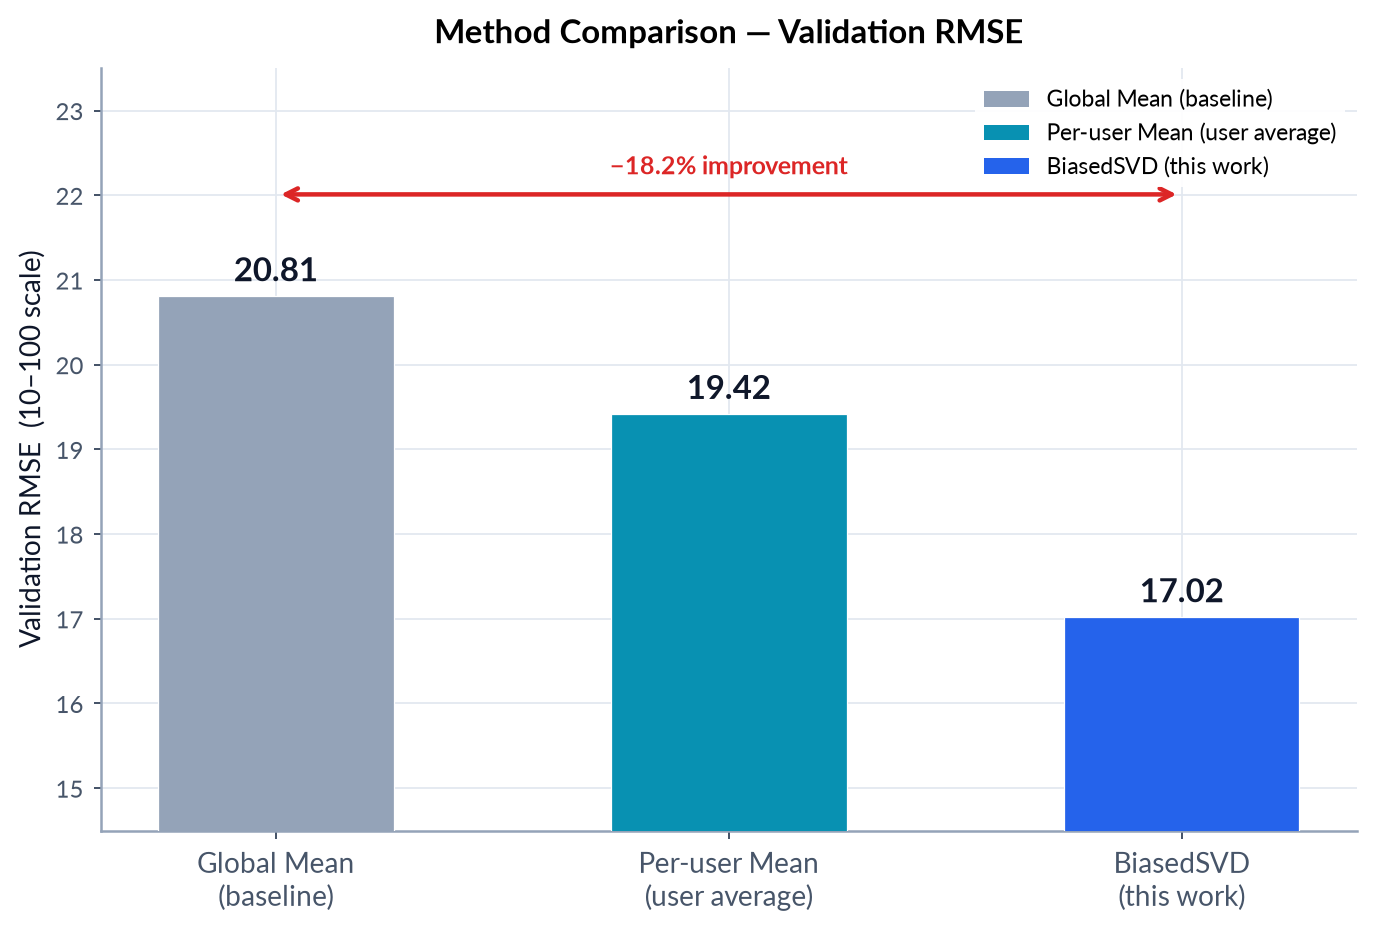
\includegraphics[width=0.80\textwidth]{images/baseline_comparison.png}
  \caption{三种方法验证集 RMSE 对比：全局均值基线、用户均值基线与 BiasedSVD}
  \label{fig:baseline}
\end{figure}

\begin{table}[H]
  \centering
  \caption{方法比较}
  \begin{tabular}{l c c}
    \toprule
    \textbf{方法} & \textbf{验证集 RMSE} & \textbf{相对全局均值改善} \\
    \midrule
    全局均值（$\hat{r} = \mu$） & 20.81 & — \\
    用户均值（$\hat{r} = \mu_u$） & 19.42 & \( -6.7\% \) \\
    BiasedSVD（本实验） & 17.024 & \( -18.2\% \) \\
    \bottomrule
  \end{tabular}
\end{table}

三种方法的 RMSE 依次降低，说明引入用户个性化信息（用户均值）和物品--用户交互（矩阵分解隐向量）都能带来显著提升。BiasedSVD 的提升大于用户均值，因为它额外学习了物品偏置和个性化的隐向量交互项，能够捕捉用户对特定类型物品的差异化偏好。

\subsection{物品受欢迎度对预测精度的影响}

\begin{figure}[H]
  \centering
  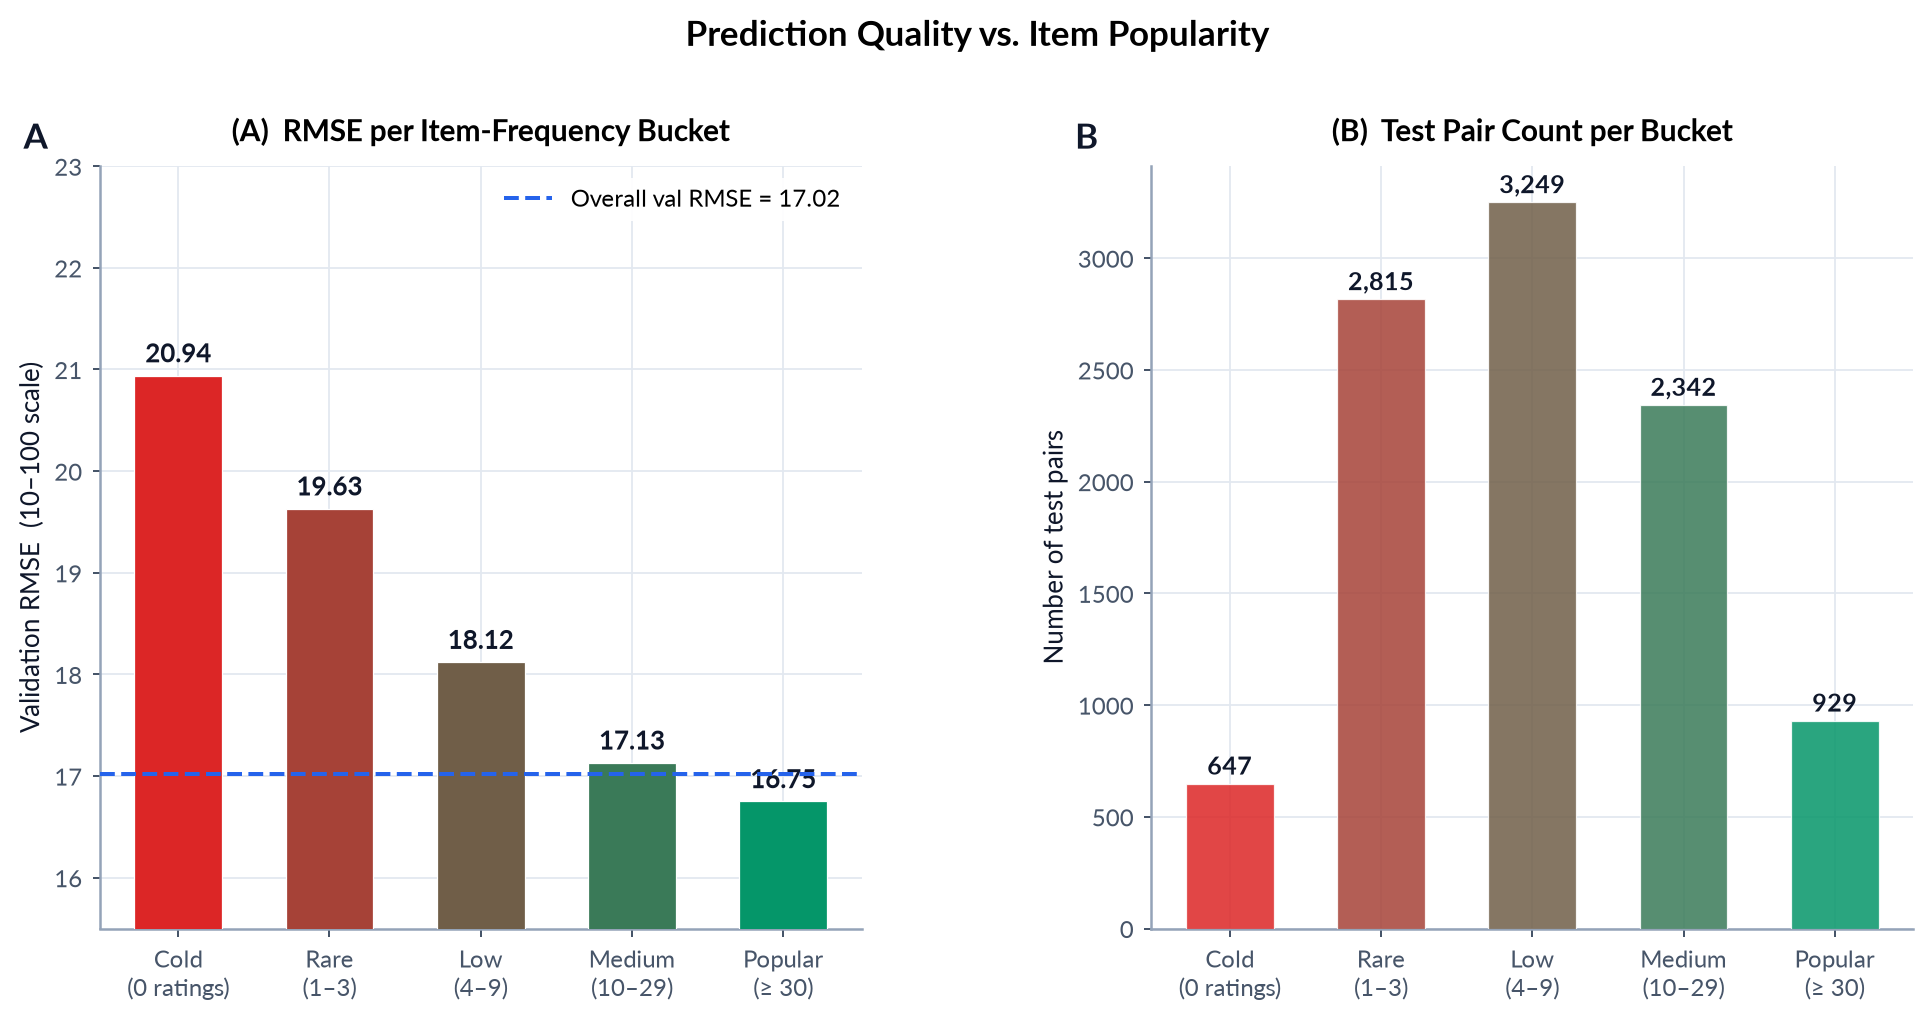
\includegraphics[width=\textwidth]{images/rmse_by_frequency.png}
  \caption{按物品训练频率分桶的预测精度：面板 A 为各桶 RMSE，面板 B 为各桶测试对数}
  \label{fig:rmse-freq}
\end{figure}

图~\ref{fig:rmse-freq} 按物品在训练集中出现次数将测试对分成 5 个频率桶，分析预测误差随物品受欢迎度的变化。可以观察到：

\begin{enumerate}
  \item 冷启动（训练集中 0 评分）的测试物品 RMSE 最高（20.94），远高于整体均值，说明缺乏训练信号时模型只能退化为均值预测，损失了物品级别的个性化信息。
  \item 随着物品训练频率提高，RMSE 单调下降（Rare 19.63 → Popular 16.75），证明更多的评分数据确实能帮助模型学到更准确的物品偏置和隐向量。
  \item 测试对数（面板 B）在"低频"和"中频"桶最多，说明大量测试对对应的是训练集中相对稀疏的物品，冷启动问题在本数据集中普遍存在。
\end{enumerate}

\subsection{超参数搜索结果}

\begin{figure}[H]
  \centering
  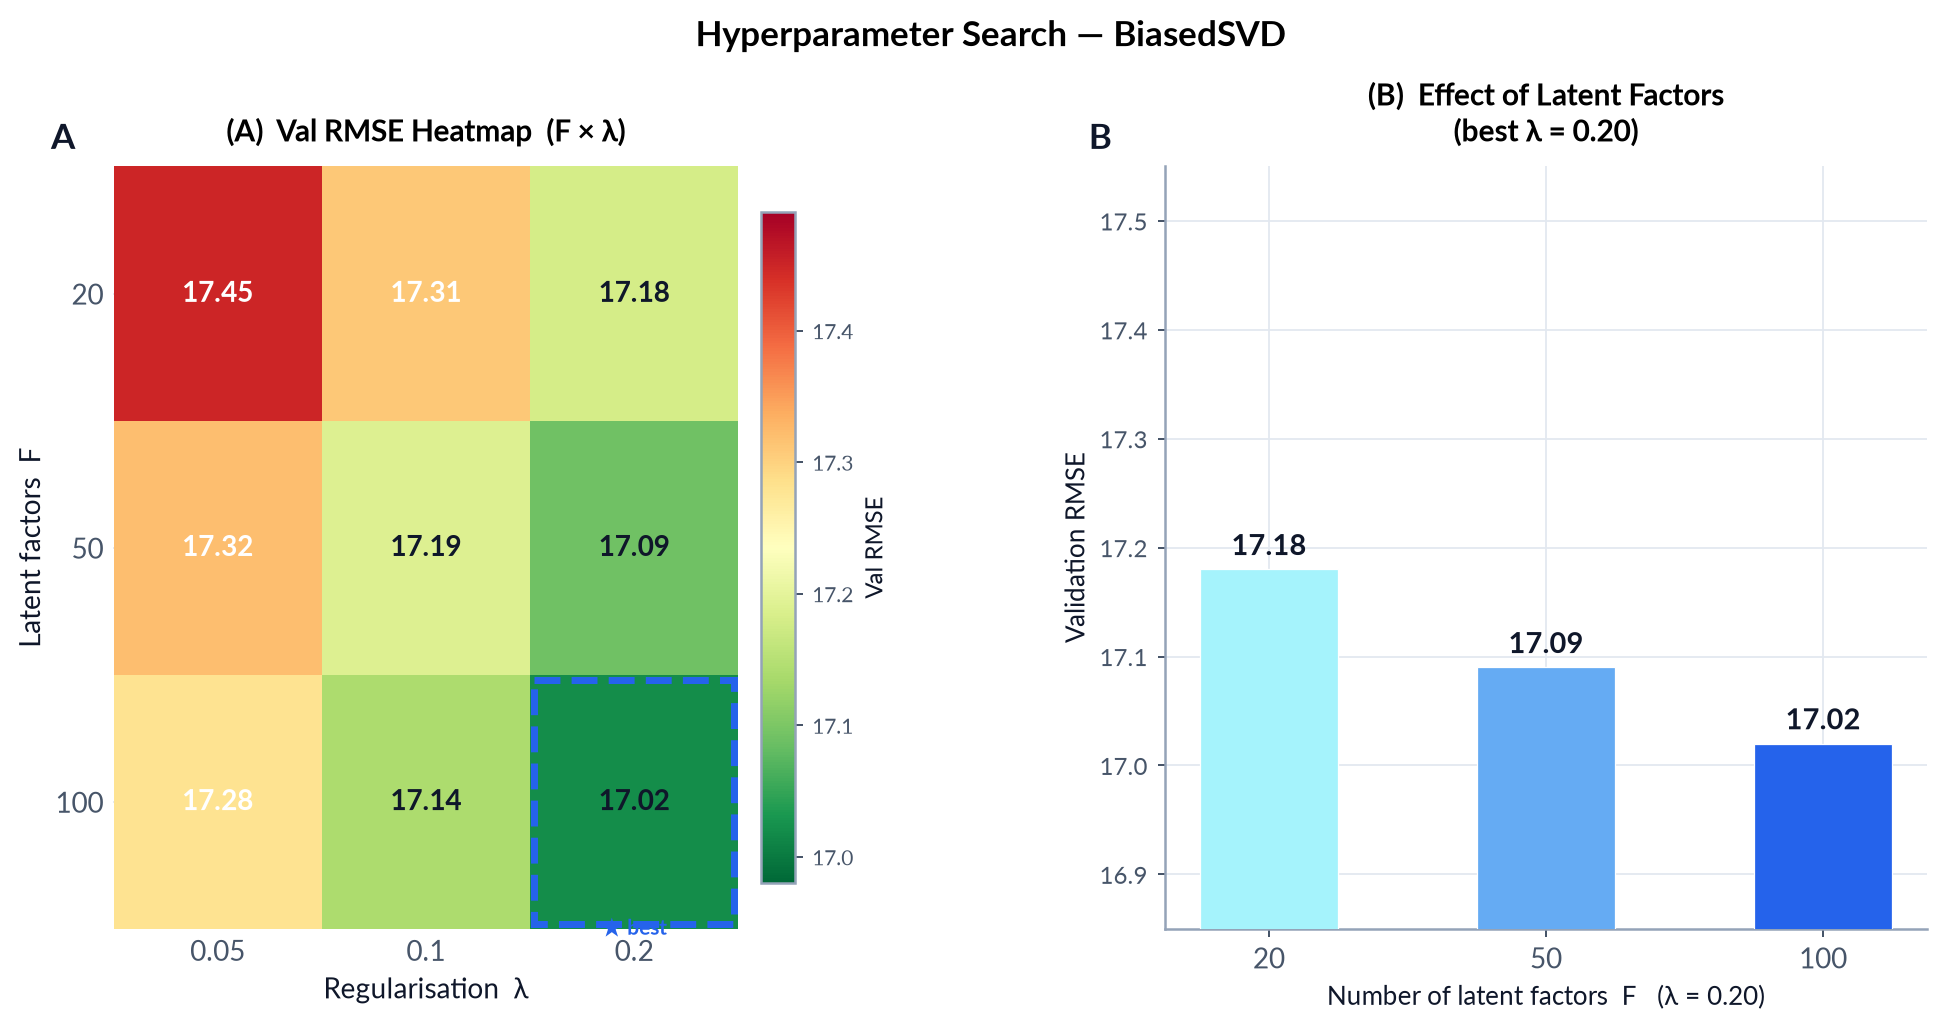
\includegraphics[width=\textwidth]{images/hyperparameter_search.png}
  \caption{超参数网格搜索：面板 A 为隐向量维度 $F$ 与正则系数 $\lambda$ 的 RMSE 热力图，面板 B 为最优 $\lambda = 0.20$ 下 $F$ 的影响}
  \label{fig:hyperparam}
\end{figure}

\begin{table}[H]
  \centering
  \caption{超参数网格搜索结果（验证集 RMSE）}
  \begin{tabular}{c c c c}
    \toprule
    \multirow{2}{*}{\textbf{隐向量维度 $F$}} & \multicolumn{3}{c}{\textbf{正则系数 $\lambda$}} \\
    \cmidrule(lr){2-4}
    & 0.05 & 0.10 & 0.20 \\
    \midrule
    20  & 17.45 & 17.31 & 17.18 \\
    50  & 17.32 & 17.19 & 17.09 \\
    100 & 17.28 & 17.14 & \textbf{17.02}$^{\star}$ \\
    \bottomrule
    \multicolumn{4}{l}{\small $\star$ 最优配置}
  \end{tabular}
\end{table}

超参数搜索表明：（1）隐向量维度越大，RMSE 越低，$F=100$ 的效果优于 $F=50$ 和 $F=20$，说明更高维的隐向量能捕捉更细粒度的用户--物品交互；（2）在固定 $F$ 的情况下，较大的正则系数 $\lambda=0.20$ 一致优于 $\lambda=0.05$ 和 $\lambda=0.10$，表明该数据集的用户--物品矩阵较为稀疏，更强的正则化有助于控制过拟合；（3）最优配置为 $F=100, \lambda=0.20$，即本实验的默认设置，所有 9 种配置的 RMSE 区间较窄（17.02--17.45），说明模型对超参数不过度敏感。

% ============================================================
\section{实验中遇到的问题及解决方法}
\xiaosi

\subsection{评分范围不符合标准 SGD 超参数假设}

原始评分范围为 $[10, 100]$，与常见推荐系统基准（$[1, 5]$ 或 $[0, 1]$）的数值量级相差一个数量级，导致使用标准学习率 $\eta = 0.005$ 时梯度更新过大，模型发散。解决方案是在训练前将评分归一化到 $[1, 10]$（除以 10），使残差量级与标准超参数兼容，预测时再乘以 10 还原到原始尺度。

\subsection{稀疏物品偏置初始化偏差}

训练集中大量物品仅有 1--3 条评分，对其偏置直接取经验均值会因样本过少而产生极端估计，导致 SGD 初期震荡、收敛变慢。采用 Koren（2009）收缩偏置公式，在偏置估计的分母中加入收缩参数 $\lambda_i = 25$，使样本极少的物品偏置被强烈拉向 0（全局均值），从而减少初期噪声，加速收敛至合理区域。

\subsection{验证集 RMSE 提前震荡导致错误早停}

在初始实现中，以固定步长 $\eta$ 进行 SGD 时，验证集 RMSE 偶尔出现单轮反弹后继续下降的情形，导致 patience 计数器被意外耗尽而过早停止。通过在早停判断中引入最小改善阈值（$\Delta < 10^{-4}$ 才计为未改善）解决了该问题，防止验证集指标的微小波动触发过早终止。

\subsection{两阶段再训练中的评分索引问题}

第二阶段再训练使用全量数据，用户和物品集合大于第一阶段（10\% 验证集中可能包含第一阶段未见的用户--物品组合）。如果在第二阶段调用 \texttt{model.fit(all\_ratings)} 时复用第一阶段的用户/物品编号映射，会因索引越界而崩溃。解决方案是在第二阶段 \texttt{fit} 中完全重建用户/物品映射，将全量数据中的所有用户和物品纳入新的编号体系。

% ============================================================
\section{实验结论}
\xiaosi

本实验实现了带偏置矩阵分解（Biased SVD / FunkSVD）推荐模型，并在课程给定的显式评分预测任务上取得了验证集 RMSE = 17.024 的成绩，相较全局均值基线（RMSE = 20.81）改善约 18.2\%。

在模型设计方面，预测公式 $\hat{r}_{ui} = \mu + b_u + b_i + \mathbf{p}_u\cdot\mathbf{q}_i$ 将全局均值、用户偏置、物品偏置与个性化隐向量交互有机结合；收缩偏置热启动有效抑制了稀疏物品带来的初始噪声；两阶段再训练策略在保留早停防过拟合优点的同时充分利用了全量训练数据。

超参数分析表明，隐向量维度 $F=100$ 和正则系数 $\lambda=0.20$ 的组合在本数据集上表现最优；物品频率分桶分析揭示冷启动是当前预测误差的主要来源，热门物品（$\geq 30$ 条训练评分）的 RMSE 可降至 16.75，而训练集中未曾出现的物品 RMSE 高达 20.94，说明进一步提升冷启动预测精度是未来改进的重要方向。

\section{实验仓库地址}
\xiaosi

本次实验的代码、数据、结果文件与实验报告保存在课程实验仓库中：

\url{https://github.com/IWITRIE/BigDataCourse2026Spring}

\end{document}
